
\subsection{VHDL et Verilog}

Verilog et VHDL (pour \english{Very High speed integrated circuit Hardware Description Language}) sont les deux langages de description de matériel (en anglais, \english{Hardware Description Language}) les plus connus. Ils ressemblent respectivement au langage \languagetoto{ADA} et \languagetoto{C}. Les HDL utilisent une méthode de description de flux de processus résultant d'un modèle de flux de données avec des informations de synchronisation. Cette méthode consiste en une abstraction au niveau des portes logiques et des transitors. Cette méthode s'appelle \english{Register-Transfer Level} (RTL) et a été définie à cause de l'explosion de la complexité des circuits électroniques depuis les années 1970 (loi de Moore). Ce niveau génère ce qu'on appelle une \english{netlist}. Les concepteurs de matériel micro-électronique avaient besoin d'une méthode de description logique des matériels numériques de plus haut niveau pour limiter la complexité de la conception et cela sans que cette dernière ne soit spécifique à une technologie en particulier. À partir de cette représentation des circuits, des représentations de plus bas niveaux et le câblage sur une carte donnée peuvent être déduits. Une \english{netlist} est indépendante de la plateforme tandis qu'un routage lui l'est.\\

Les HDL permettent de décrire un circuit électronique tant au niveau comportemental que structurel, c'est-à-dire les flux de signaux transitant entre les différents registres. C'est pour cette simplification dans la conception et l'utilisation des matériels que les HDL sont largement utilisés dans l'industrie.\\
\begin{figure}[h!]
\centering
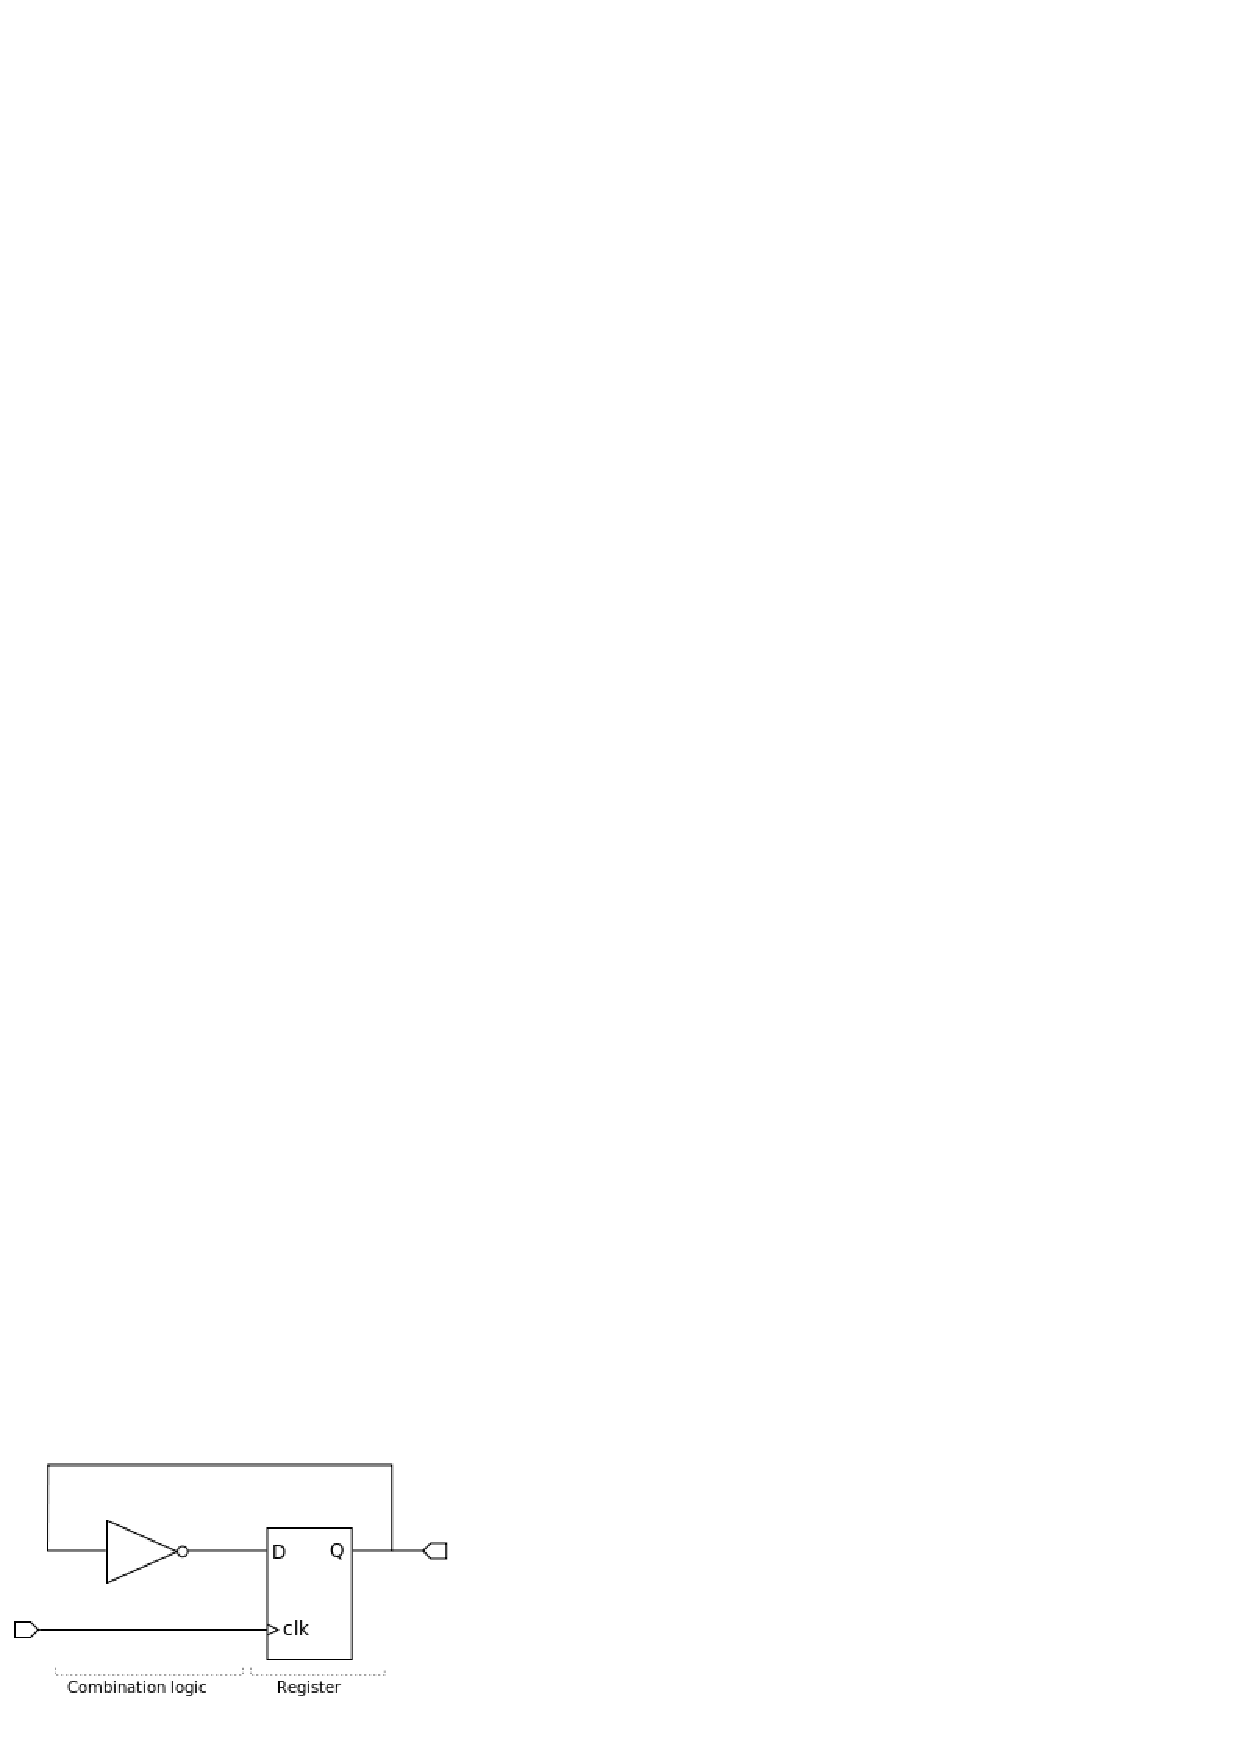
\includegraphics[scale=0.9]{rtl_example.png}
\caption{Bascule D}
\label{BasculeD}
\end{figure}
La figure \ref{BasculeD} montre comment est représenté un circuit. Nous constatons qu'il est ici totalement fait abstraction de la manière avec laquelle ce dernier est câblé. Nous ne connaissons que ce qui est en entrée et sortie de ce dernier. Un HDL décrira, quant à lui, le {\og}comportement{\fg} externe, général du circuit.\\
L'une des principales différences entre les HDL et les langages de programmations traditionnels est qu'avec un HDL il est possible de modéliser plusieurs processus parallèles. Par exemple, un changement dans un des processus pourra donc déclencher une mise à jour dans les autres processus.\\
\\
VHDL et Verilog ont chacun leurs atouts listés non exhaustivement ici :
\begin{itemize}
\item VHDL :
    \begin{itemize}
    \item ce langage a été conçu pour aider la conception et la spécification au niveau d'un système électronique,
    \item il est plus souple que Verilog car permet, entre autre, à l'utilisateur de définir ses types, ses configurations, etc.
    \end{itemize}
    \vspace{10px}
    \item Verilog :
    \begin{itemize}
    \item conçu de base pour les concepteurs de matériel développant des \fpgas{} et ASICs
    \item parfait pour convertir des types de données de vecteurs de bits vers des notations arithmétiques,
    \item existence de supports compréhensibles pour la conception numérique de bas niveau.
    \end{itemize}
\end{itemize}
\vspace{10px}
VHDL et Verilog sont tous les deux des standards IEEE : \textit{IEEE standard 1076-1987}
\cite{IEEE_VHDL_87}
en 1987 puis \textit{IEEE standard 1076-1993}
\cite{IEEE_VHDL_93}
 en 1993 après une mise à jour pour VHDL. Il a ensuite été mis à jour régulièrement pour arriver, en 2008 au standard \textit{IEEE 1076}
\cite{IEEE_VHDL}
 (VHDL 4.0) qui est la dernière version en date. Quant à Verilog, il est devenu un standard en 1995 : \textit{IEEE standard 1364-1995}
\cite{IEEE_VERILOG_1995}
et a été mis à jour deux fois depuis : en 2001 \textit{IEEE Standard 1364-2001}
\cite{IEEE_VERILOG_2001}
(Verilog 2001) qui corrigera de nombreux problèmes puis en 2005 \textit{IEEE Standard 1364-2005}
\cite{IEEE_VERILOG_2005}
(Verilog 2005) qui corrigea quelques bogues.\\

Historiquement, VHDL a été développé pour l'armée de l'air des États-Unis d'Amérique (contrat \textit{F33615-83-C-1003}) par \brand{Intermetrics, Inc.}, \brand{Texas Instruments} et \brand{IBM}. \brand{Intermetrics, Inc.} fournissait les experts en langage de programmation et était aussi le maître d'\oe{}uvre du projet. \brand{Texas Instruments} se concentrait sur la partie expertise en conception de puces. \brand{IBM} quant à elle fournissait les experts en conception de systèmes informatiques. C'était donc un projet de envergure (comme \languagetoto{ADA} par exemple). Verilog a quant à lui été démarré en 1984 par \brand{Gateway Design Automation Inc.} puis rendu disponible au grand public en 1990 par \brand{Cadence}.

\subsection{Les autres langages HDL existants}

Il existe bien d'autres langages que Verilog et VHDL. Altera HDL (AHDL) est un langage propriétaire d'\brand{Altera}, Hydra est fondé sur \languagetoto{Haskell}, MyHDL est fondé sur \languagetoto{Python} ou encore RHDL qui s'appuie sur \languagetoto{Ruby}. Un autre langage appelé \languagetoto{SystemC} est très utilisé dans l'industrie. Cependant, ce dernier n'est pas un langage à part entière puisqu'il utilise un ensemble de classes \languagetoto{C++} fournissant les outils nécessaires à la modélisation du matériel. 
